\documentclass[a4paper, 14pt]{article} %{article}
\usepackage{arxiv}

\usepackage[utf8]{inputenc}
\usepackage[english, russian]{babel}
\usepackage[T2A]{fontenc}
\usepackage{url}
\usepackage{booktabs}
\usepackage{amsfonts}
\usepackage{nicefrac}
\usepackage{microtype}
\usepackage{lipsum}
\usepackage{graphicx}
\usepackage{natbib}
\usepackage{doi}
\usepackage[hidelinks]{hyperref}
\usepackage{subfigure}
\usepackage{bm}
\usepackage{fontawesome}
\usepackage{verbatim}
\usepackage{comment}
\usepackage{enumitem}
\usepackage{amsmath}
\usepackage{diagbox}


\title{Методы машинного обучения для функционального картирования мозга}

\author{Арина~Чумаченко  \\
	МФТИ, Сколтех\\
	\texttt{chumachenko.as@phystech.edu} \\
	%% examples of more authors
	\And
	Максим Шараев \\
	Сколтех\\
	\texttt{M.Sharaev@skoltech.ru} \\
	%% \AND
	%% Coauthor \\
	%% Affiliation \\
	%% Address \\
	%% \texttt{email} \\
	%% \And
	%% Coauthor \\
	%% Affiliation \\
	%% Address \\
	%% \texttt{email} \\
	%% \And
	%% Coauthor \\
	%% Affiliation \\
	%% Address \\
	%% \texttt{email} \\
}
\date{}

\renewcommand{\shorttitle}
% {\textit{arXiv} Template}

%%% Add PDF metadata to help others organize their library
%%% Once the PDF is generated, you can check the metadata with
%%% $ pdfinfo template.pdf
\hypersetup{
pdftitle={A template for the arxiv style},
pdfsubject={q-bio.NC, q-bio.QM},
pdfauthor={David S.~Hippocampus, Elias D.~Striatum},
pdfkeywords={First keyword, Second keyword, More},
}

\begin{document}
\maketitle

\begin{abstract}
    В исследованиях функциональной нейровизуализации для изучения функций мозга обычно используются подходы, основанные на задачах или состоянии покоя. 
Подходы, основанные на состоянии покоя, обеспечивают гибкость и масштабируемость при оценке функций мозга, в то время как методы, основанные на задачах, обеспечивают качественные возможности локализации. 
Одной из таких моделей является BrainsurfCNN, полностью сверточная модель нейронной сети на основе поверхностного слоя коры головного мозга. 
Существует также другой подход к решению проблемы функционального картирования мозга - это пространственно-ограниченный независимый компонентный анализ (ICA) для функциональной магнитно-резонансной томографии (fMRI), который использует пространственную информацию в рамках ограниченного ICA с обучением по фиксированной точке. 
Основная цель этой работы заключается в решении задачи сегментации функциональных областей fMRI снимком головного мозга, то есть в создании модели, которая принимает в качестве входных данных 4D-тензор характеристик мозга и возвращает карту с необходимыми метками. 
В частности, целью является снижение индексности данных о функциональной связности в состоянии покоя при построении карт активации.

\end{abstract}


\keywords{: \, CNN на основе поверхностного слоя \and fMRI в состоянии покоя \and ICA с фиксированной точкой}


\section{Введение}

Функциональная магнитно-резонансная томография (fMRI), основанная на задачах, имеет решающее значение для изучения когнитивных, эмоциональных и двигательных процессов в мозге человека (\cite{anticevic2008 comparing, besle2013single, schaefer2018local}).
Это дает ценную информацию о функциях мозга и позволяет получать биомаркеры для различных поведенческих показателей  (\cite{mcnab2008prefrontal}, \cite{risk2007neural}, \cite{nijhof2015simulating}).
Тем не менее, tfMRI требует тщательного проектирования и обширной предметной подготовки (\cite{church2010task}, \cite{rosazza2018pre}).
В то время как fMRI в состоянии покоя (rsfMRI) завоевала популярность благодаря своей простоте и устойчивости к ошибкам (\cite{power2014studying}, \cite{dubois2016building}).
RsfMRI выявляет крупномасштабные мозговые сети, связанные с различными когнитивными процессами, и может отражать индивидуальные особенности и психологические факторы.
Эта работа сосредоточена на прогнозировании активности мозга, связанной с конкретной задачей, по функциональным связям в состоянии покоя у здоровых индивидов.
Несмотря на методологические различия, tfMRI и rsfMRI используют сходные нейронные процессы, что предполагает предсказуемость.
Важно отметить, что предыдущим моделям линейной регрессии не хватало точности предсказания.
В этой работе будет рассмотрен модель глубокого обучения BrainSurfCNN, использующая современные инструменты для устранения этого недостатка.

Несмотря на то, что машинное обучение продвинулось вперед в различных областях, его применение в исследованиях функциональной магнитно-резонансной томографии (fMRI) отстает, главным образом, из-за ограничений, которые присутствуют у высококачественных наборов данных.
Наборы данных нейровизуализации, как правило, довольно малы и содержат шумы, что создает проблемы для обучения высокопроизводительных нейронных сетей.
Чтобы решить эту проблему, в этой работе представлена BrainSurfCNN -- поверхностная нейронная сеть, которая предназначена для прогнозирования различий в задачах в сравнении с состоянием покоя.
В отличие от предыдущих традиционных подходов, работающих с трехмерными изображениями или двумерными срезами, этот метод использует поверхностное представление, используя геометрию коры головного мозга и сохраняя целостность сигнала.

\section{Метод}

\subsection{Многоканальные vertex‐to‐ROI функциональные коннектомы}

Входными данными для моделей прогнозирования являются функциональные коннектомы, представленные в виде многоканальных данных, прикрепленных к вершинам икосаэдрической сетки.
На рис.\ref{BrSurf2} показана конструкция многоканальных функциональных коннектомов vertex-to-ROI (из вершины в интересующий регион), используемых в наших экспериментах.
Такая функциональная связь задается формулой:

\begin{figure}
\centering
\includegraphics[scale=0.4]{fig/fig1.png}
\caption{\footnotesize{Многоканальные функциональные коннектомы vertex-to-ROI, вычисленные на основе rsfMRI}}
\label{BrSurf2}
\end{figure}

\begin{equation}
    \boldsymbol{r}_{ij} = corr(\boldsymbol{t}_i, \bar{\boldsymbol{t}}_j)
\end{equation}

где $\boldsymbol{r}_{ij}$ представляет собой функциональную связность между $i$-ой вершиной поверхности и $j$-ым интересующим регионом, и вычисляется как коэффициент корреляции Пирсона $corr(.)$  между временными рядами $\textbf{t}_i$ rsfMRI в $i$-й вершине и средним значением временных рядов $\bar{\textbf{t}}_j$ для $j$-го интересующего региона.
В наших экспериментах шаблоном поверхности является fs$\_$LR шаблон с $32 492$ вершинами (\cite{van2012parcellations}).
ROI -- это парсели (регионы), полученные на основе группового независимого компонентного анализа (ICA) (\cite{smith2013resting}), в котором $50$ компонентов были рассчитаны на основе временных рядов fMRI в состоянии покоя объектов обучения (поэтому испытуемые были исключены из ICA).
Каждой вершине присваивается метка участка, соответствующая компоненту с наибольшим значением z-балла в данном местоположении.
Из всех значений ROI $42$ лежат на кортикальной поверхности.
Коннектомы каждого объекта из двух полушарий могут быть объединены, в результате чего получается единая входная икосаэдрическая сетка с количеством каналов, в два раза превышающим количество ROI.
Следовательно, результирующий функциональный коннектом каждого субъекта представляет собой сетку из $32,492$ вершин с $84$ каналами.

Использование корреляции временных рядов rsfMRI между вершинами и ROI для определения функциональной связности мозга является широко распространенной практикой в нейровизуализационном анализе.
По сравнению с функциональными коннектомами ROI-to-ROI и плотными функциональными коннектомами vertex-to-vertex, функциональные коннектомы vertex-to-ROI обеспечивают баланс между представлением с высоким пространственным разрешением, необходимым для моделей прогнозирования, и при этом остаются выполнимыми с точки зрения вычислений.


\subsection{Модель BrainSurfCNN}

\begin{figure}
\centering
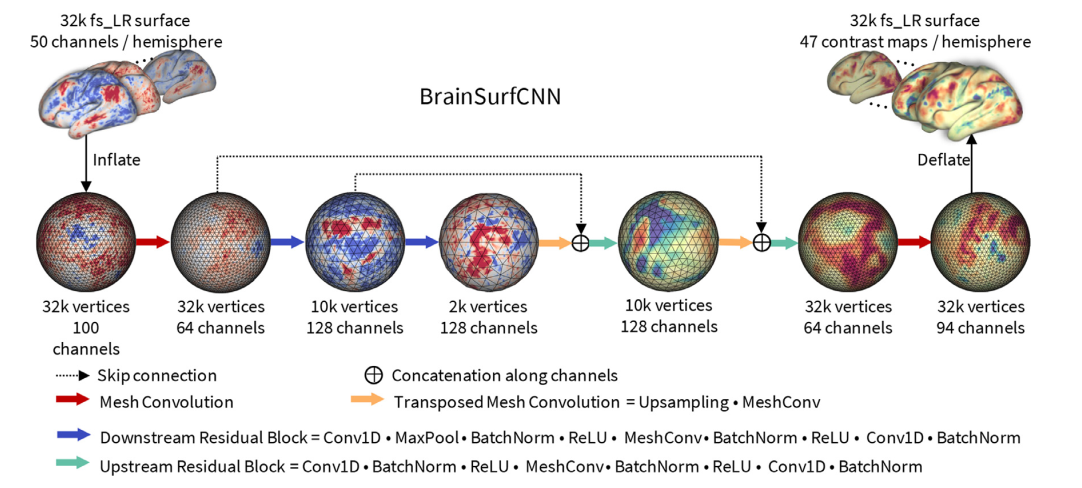
\includegraphics[scale=0.5]{fig/BrainSurfCNN.png}
\caption{\footnotesize {Модель BrainSurfCNN}}
\label{BrSurf}
\end{figure}

На рис.\ref{BrSurf} показана рассматриваемая модель BrainSurfCNN для прогнозирования различий между задачами и функциональными коннектомами в состоянии покоя.
BrainSurfCNN основана на архитектуре UNet (\cite{ronneberger2015u}) и использует сферическое сверточное ядро для работы со сферической сеткой.
Наиболее заметной особенностью архитектуры UNet являются пропускные соединения, которые копируют функции из блока кодирования (выходы из нижних блоках на рис.\ref{BrSurf}) на входы блока декодирования (входы для верхних блоках на рис.\ref{BrSurf}).
Входная и выходная поверхности представляют собой шаблоны fs$\_$LR с $32,492$ вершинами (поверхность fs$\_$LR $32$k) на каждое полушарие мозга.
Левое и правое полушария симметричны в атласах fs$\_$LR, т.е. одинаковый индекс вершины в обоих полушариях соответствует противоположным гомологам.
Таким образом, коннектомы каждого объекта из двух полушарий могут быть объединены, в результате чего получается единая входная икосаэдрическая сетка с количеством каналов, в два раза превышающим количество ROI.
На выходе BrainSurfCNN также представляет собой многоканальную икосаэдрическую сетку, в которой каждый канал соответствует контрасту для одной задачи МРТ.
% Эта настройка многозадачного прогнозирования способствует распределению веса между прогнозируемыми контрастами.


\subsection{Функция потерь}

В процессе обучения модели BrainSurfCNN минимизируется реконструктивно-контрастивная функция потерь (RC loss, \cite{koch2015siamese}). 
RC loss связан с метрическим обучением, и также применим к задаче генерации изображений в области нейронауки.

Дан минибатч из $N$ сэмплов: $B=\{\textbf{x}_i\}$., в котором
$\textbf{x}_i$ представляет собой  целевое многоконтрастное изображение объекта $i$, пусть $\hat{\textbf{x}}_i$ определяет соответствующее прогнозируемое изображение контраста. Тогда RC loss можно выразить как:
\begin{equation}
    \mathcal{L}_R = \frac{1}{N} \sum\limits_{i=1}^N d(\hat{\textbf{x}}_i, {\textbf{x}}_i),
\end{equation} 

\begin{equation}
    \mathcal{L}_C = \frac{1}{(N^2-N)/2} \sum\limits_{\substack{\textbf{x}_j \in B_i, \\ j\neq i}} d(\hat{\textbf{x}}_i, {\textbf{x}}_j),
\end{equation}

\begin{equation}
    \mathcal{L}_{RC} = [\mathcal{L}_R - \alpha]_+ + [\mathcal{L}_R - \mathcal{L}_C + \beta]_+,
\end{equation}
где $d(.)$ является функцией потерь (например, $l_2$-нормой, которая и была использована в экспериментах).
$\mathcal{L}_R, \alpha$ -- потери и отступ (margin) для одного и то же объекта (R loss).
$\mathcal{L}_C, \beta$ -- потери и отступ (margin) для разных объектов (C loss). 
В совокупности получаем $\mathcal {L}_{RC}$, что приводит к тому, что ошибка по одному и тому же объекту $\mathcal{L}_{R}$ находится в пределах допустимого значения $\alpha$, в то время как разница по разным объектам $\mathcal{L}_{C}$ является такой большой, что $(\mathcal{L}_C-\mathcal{L}_R) > \beta$.
% Как были установлены $\alpha$ и $\beta$ на практике, описано ниже.


\subsection{Основная модель (baseline)}
\subsubsection{Линейная регрессия}

Основная модель линейной регрессии (\cite{tavor2016task}) представлена как:
\begin{equation}
    \boldsymbol{y}_i^k = \boldsymbol{X}_i^k \boldsymbol{\beta}_i^k,   
\end{equation}
где $\boldsymbol{y}_i^k, \boldsymbol{X}_i^k,  \boldsymbol{\beta}_i^k$ являются патерном активации, входными признаками и регрессором для $k$-го участка в $i$-м объекте, соответственно.
Для вычисления модели линейной регрессии была использована парцелляция из $50$ компонентов, полученная из ICA и предоставленная HCP. 

$\boldsymbol{y}_i^k$ является вектором длины $n_k$, где $n_k$ -- количество вертексов в $k$-ом парселе в обоих полушариях мозга.
$\boldsymbol{X}_i^k$ является функциональной матрицей связности размером  $n_k \times M$, где каждый элемент был вычислен как корреляция Пирсона между вертексом и средним временных рядов каждого из $M$ интересующих регионов (те же временные ряды были использованы для вычисления входных данных модели BrainSurfCNN).
 
Линейная модель была подобрана для каждого участка и каждого контраста задач каждого объекта обучения.
Таким образом, после обучения заданному контрасту задач для каждого участка существует отдельная линейная модель, подобранная для каждого объекта обучения.
Для вычисления прогнозов по данным полученные веса линейных моделей были усреднены по всем объектам, чтобы получить единую прогностическую модель для каждого парселя.
% Отметим, что это соответствует сборке линейных моделей по всем испытуемым.

Предсказанный патерн активации $\hat{\boldsymbol{y}}_{\text{test}}^k$ $k$-го парселя невидимого (не участвовавшего в обучении) объекта исследования вычисляется как:
\begin{equation}
\hat{\boldsymbol{y}}_{\text{test}}^k = {\boldsymbol{X}}_{\text{test}}^k \bar{\boldsymbol{\beta}}^k = {\boldsymbol{X}}_{\text{test}}^k \frac{1}{N_{\text{train}}} \sum_{i=1}^{N_{\text{train}}} {\boldsymbol{\beta}}_i^k = \frac{1}{N_{\text{train}}} \sum_{i=1}^{N_{\text{train}}} {\boldsymbol{X}}_{\text{test}}^k {\boldsymbol{\beta}}_i^k,
\end{equation} 
где $\bar{\boldsymbol{\beta}}^k$ представляет собой усреднённые веса моделей линейной регрессии для $k$-го парселя, вычисленного по $N_\text{train}$ объектам обучения.


\subsubsection{Усреднённые по группе контрасты}
Разная степень вариабельность между индивидами проявляется в различных контрастах задач.
Такая вариабельность была интересна для этого исследования.
Поэтому были использованы средние значения по группе в качестве наивного ориентира.
Усреднённые по группе контрасты также отражают наиболее характерные особенности карты активации, зависимые от условий задачи, что должна учитывать модель прогнозирования.


\subsubsection{Повторяющиеся контрасты}
В этой работе были использованы повторные fMRI-сканирования (при их наличии) для количественной оценки надежности целевых карт контрастов и оценки характеристик прогнозирования модели BrainSurfCNN и новной модели.
Повторные контрасты сравнивались с первоначальными контрастами как с точки зрения общего соответствия (измеренного с помощью игральных костей), так и в задаче идентификации объекта.


\subsection{Метрика качества}
Показатель Dice (\cite{dice1945measures}) используется для измерения степени совпадения между прогнозируемым контрастом и целевой картой контрастности для заданного процента наиболее активированных вершин.
При заданном пороговом значении $x\%$, показатель Dice вычисляется как:
\begin{equation}
    Dice(x) = \frac{2 | Prediction(x) \cap Target(x)|}{| Prediction(x) | + | Target(x)|},
\end{equation}
где $| Prediction(x) |$ определяет  количество топ-$x\%$ наиболее активированных вершин на прогнозируемой карте контрастности, $| Target(x)|$ $| Target(x)|$ определяет количество топ-$x\%$ наиболее активированных вершин в контрасте, и $| Prediction(x) \cap Target(x)|$ определяет количество вершин, которые перекрывают прогнозируемую и целевую карты при заданном пороговом значении. 

При более низком пороговом значении (например, при $5\%$ наиболее активированных вершин) показатель Dice измеряет соответствие мелких деталей между целевым и прогнозируемым контрастами.
При более высоких пороговых значениях (например, $50\%$ наиболее активированных вершин) этот показатель количественно определяет глобальное соответствие анатомических распределений.
Интегрируя показатели Dice по ряду пороговых значений (от $5\%$ до $50\%$ от наиболее активированных вершин с интервалом в $5\%$), мы получаем итоговый показатель - площадь под кривой Dice (Dice AUC) -
для оценки качества предсказания модели.



\section{Вычислительный эксперимент}

\subsection{Датасет}

В этой работе для экспериментов с большим набором данных были использованы предварительно обработанные и предварительно очищенные МРТ в состоянии покоя (3-Tesla rsfMRI) и МРТ для задач (tfMRI) для 1200 испытуемых из проекта Human Connectome Project (HCP, \cite{glasser2013minimal}). 
Сбор и предварительная обработка набора данных были описаны в работах \cite{glasser2013minimal}, \cite{smith2013resting} и \cite{barch2013function}. 
Данные rsfMRI были получены за четыре 15-минутных цикла, каждый из которых включал $1200$ временных точек для каждого испытуемого. 
HCP также реализовал парцелляции на уровне группы, полученные на основе пространственной ICA. 
В этой работе были использованы ROI из $50$-компонентной парцелляции для вычисления функциональных коннектомов. 
Данные tfMRI, полученные HCP, содержат $86$ контрастов из $7$ областей задач (\cite{barch2013function}), а именно: WM (working memory), GAMBLING,
MOTOR, LANGUAGE, SOCIAL RELATIONAL и EMOTION. 
После исследования \cite{tavor2016task} были исключены избыточные отрицательные контрасты, в результате чего было получено $47$ уникальных контрастов. 
Из $1200$ пациентов, прошедших HCP, у $46$ пациентов также были повторные данные 3T-МРТ. 
Включая только испытуемых, у которых были проведены все $4$ rsfMRI-сканирования и $47$ контрастных tfMRI-исследований, набор данных включал $919$ испытуемых для обучения/проверки и $39$ независимых испытуемых (с повторными сканированиями) для оценки.


\subsection{Основной эксперимент}

На рис.\ref{BrSurf3} показана корреляция предсказания моделей с наблюдаемыми картами контрастности того же объекта.
На последующих рисунках показаны предсказанные контрасты заданий, определяемые как те, у которых средняя корреляция между тестом и повторным тестированием по всем испытуемым больше, чем средняя корреляция по всем испытуемым и контрастам.
На рис.\ref{BrSurf4} показана поверхностная визуализация двух контрастов заданий для двух испытуемых.
В то время как средние значения по группе соответствуют грубому характеру индивидуальных контрастов, контрасты, характерные для конкретного объекта, демонстрируют мелкие детали, которые воспроизводятся при повторном тестировании, но стираются в средних показателях по группе.
С другой стороны, предсказания с помощью модели линейной регрессии не учитывали общие особенности активации, характерные для некоторых контрастов.
В целом, прогноз модели BrainSurfCNN неизменно давал самую высокую корреляцию с индивидуальными контрастами tfMRI, приближаясь к верхней границе контрольного показателя повторного тестирования испытуемых.

\begin{figure}
\centering
\includegraphics[scale=0.425]{fig/fig3.png}
\caption{Корреляция между предсказанными и истинными индивидуальными контрастами. LANG, REL, SOC, EMO, WM, и GAMBL являются сокращениями от LANGUAGE, RELATIONAL, SOCIAL, EMOTION, WORKING MEMORY и GAMBLING соответственно.}
\label{BrSurf3}
\end{figure}



\begin{figure}
\centering
\includegraphics[scale=0.55]{fig/fig4.png}
\caption{{Визуализация поверхности для сравнения 2-х заданий у 2-х испытуемых. В крайнем правом столбце приведены средние значения контрастов по группе для сравнения.}}
\label{BrSurf4}
\end{figure}


Матрицы были нормализованы для наглядности, чтобы учесть более высокую вариабельность между истинными и прогнозируемыми контрастами.
Все матрицы имеют диагональное преобладание, что указывает на то, что индивидуальные прогнозы, как правило, наиболее близки к контрастам у одних и тех же испытуемых.

\begin{figure}
\centering
\includegraphics[scale=0.55]{fig/fig5.png}
\caption{{Нормализованные корреляционные матрицы прогнозируемых и истинных контрастов между испытуемыми для трёх заданий и 39 испытуемых.}}
\label{BrSurf5}
\end{figure}


\begin{figure}
\centering
\includegraphics[scale=0.5]{fig/fig6.png}
\caption{{Точность прогнозов для индивида в 23 надежно прогнозируемых задачах.}}
\label{BrSurf6}
\end{figure}

При всех достоверных картах контрастности, карты контрастности, предсказанные моделью BrainSurfCNN, имеют неизменно лучшую точность идентификации объекта по сравнению с моделью линейной регрессии, показанной на рис.\ref{BrSurf5}, и более четкими диагоналями на рис.\ref{BrSurf6}.

\section{Заключение}

В этой работе был применён подход для индивидуального прогнозирования контрастов в задачах по функциональным коннектомам с использованием поверхностного CNN.
В ходе экспериментов ранее опубликованная базовая модель достигла более низких значений корреляции, чем средние значения по группе, что может быть связано с моделированием на уровне ROI, при котором не учитывается соответствующий сигнал от остальной части мозга.
Исследование мозга дало прогнозы, которые в целом были сильно коррелированы с результатами исследования МРТ отдельных людей и были весьма специфичны для них.
Также в качестве функции потерь была использована реконструктивно-контрастивную потеря (RC loss), которая значительно улучшила распознаваемость объекта, что соответствует верхней границе теста и повторного тестирования.

Существует несколько расширений существующего подхода, работа над которыми представляет продолжение этого исследования.
Во-первых, можно распространить прогнозы на подкорковые и мозжечковые компоненты мозга.
Во-вторых, повреждение мозга и потеря памяти могут быть применены к другим областям прогнозирования, где важна специфика индивида, например, при индивидуальных траекториях развития заболеваний.
Кроме того, прогнозирование модели BranSurfCNN может быть внедрено в инструменты контроля качества для tfMRI, когда данные повторного тестирования недоступны.

Эксперименты показывают, что нейронная сеть, основанная на работе с поверхность головного мозга человека, может эффективно извлекать полезные многомасштабные характеристики из функциональных коннектомов для прогнозирования контрастов tfMRI, которые очень специфичны для конкретного человека.


\bibliographystyle{unsrtnat}
\bibliography{references}

\end{document}